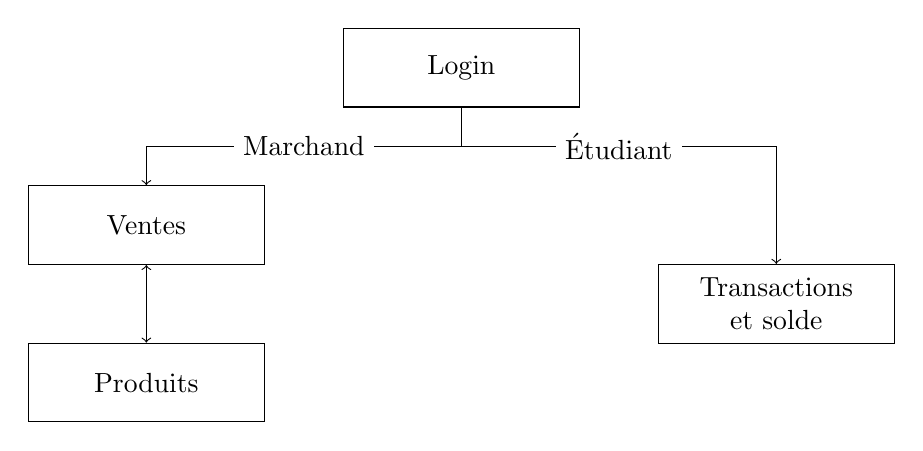
\begin{tikzpicture}[minimum height=1cm, minimum width=3cm, align=center]
	\node[draw] (prod) at (0,0) {Produits};
	\node[draw] (sales) at (0,2) {Ventes};
	\node[draw] (trans-solde) at (8,1) {Transactions \\ et solde};
	\node[draw] (login) at (4,4) {Login};
	%%%%%%%%%%%%%
	\draw[<->] (prod) -- (sales);
	\draw (login) -- (4,3);
	\draw (4,3) -- node[midway, fill=white, minimum size=0cm] {Marchand} (0,3);
	\draw (4,3) -- node[midway, fill=white, minimum size=0cm] {Étudiant} (8,3);
	\draw[->] (0,3) -- (sales);
	\draw[->] (8,3) -- (trans-solde);
\end{tikzpicture}